\documentclass[letterpaper,12pt]{article}
\usepackage{array}
\usepackage{geometry}

\geometry{letterpaper,tmargin=1in,bmargin=1in,lmargin=1.25in,rmargin=1.25in}
%\renewcommand\headrulewidth{2pt}
%\renewcommand\footrulewidth{2pt}
\usepackage{amsmath}
\usepackage{amssymb}
\usepackage{amsthm}
\usepackage{harvard}
\usepackage{setspace}
\usepackage{float,color}
\usepackage[pdftex]{graphicx}
\usepackage{hyperref}
\hypersetup{colorlinks,linkcolor=red,urlcolor=blue}
\theoremstyle{definition}
\newtheorem{theorem}{Theorem}
\newtheorem{acknowledgement}[theorem]{Acknowledgement}
\newtheorem{algorithm}[theorem]{Algorithm}
\newtheorem{axiom}[theorem]{Axiom}
\newtheorem{case}[theorem]{Case}
\newtheorem{claim}[theorem]{Claim}
\newtheorem{conclusion}[theorem]{Conclusion}
\newtheorem{condition}[theorem]{Condition}
\newtheorem{conjecture}[theorem]{Conjecture}
\newtheorem{corollary}[theorem]{Corollary}
\newtheorem{criterion}[theorem]{Criterion}
\newtheorem{definition}[theorem]{Definition}
\newtheorem{derivation}{Derivation} % Number derivations on their own
\newtheorem{example}[theorem]{Example}
\newtheorem{exercise}[theorem]{Exercise}
\newtheorem{lemma}[theorem]{Lemma}
\newtheorem{notation}[theorem]{Notation}
\newtheorem{problem}[theorem]{Problem}
\newtheorem{proposition}{Proposition} % Number propositions on their own
\newtheorem{remark}[theorem]{Remark}
\newtheorem{solution}[theorem]{Solution}
\newtheorem{summary}[theorem]{Summary}
\numberwithin{equation}{section}
\bibliographystyle{aer}
\newcommand\ve{\varepsilon}
\newcommand\boldline{\arrayrulewidth{1pt}\hline}

\def\changemargin#1#2{\list{}{\rightmargin#2\leftmargin#1}\item[]}
\let\endchangemargin=\endlist 

\usepackage{graphicx}
\graphicspath{ {images/} }

\usepackage{enumerate}
%\usepackage[shortlabels]{enumerate}
\setlength{\parindent}{24pt}
%\renewcommand{\baselinestretch}{2.0}
\usepackage{lipsum} % just for the example
\makeatletter
\newcommand{\verbatimfont}[1]{\renewcommand{\verbatim@font}{\ttfamily#1}}
\makeatother
%\usepackage{enumitem}


\verbatimfont{\small}%


\begin{document}

\begin{flushleft}
   \textbf{\Large{Problem Set \#6}} \\
   MACSS 40000 \\
   Luxi Han, 10449918\\
\end{flushleft}


\noindent \textbf{\large Problem 1}\par
	\begin{enumerate}[(a)]
		\item \quad \\
		The plot is shown as following:\\
		\begin{figure}[h]
    			\centering
			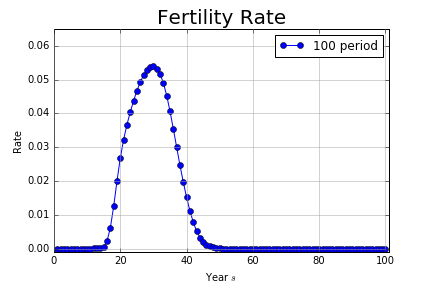
\includegraphics[width=12cm]{fert_rate1}\
    			\textbf{\caption{Fertility Rate for 100 Periods}}
		\end{figure}\par
	
	The above graph is the fertility rate for total period equal to 100 periods.\\
	
		\item \quad \\
		\begin{figure}[H]
    			\centering
			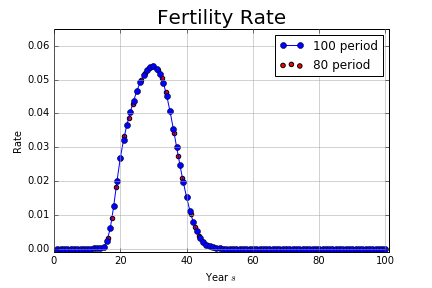
\includegraphics[width=12cm]{fert_rate2}\
    			\textbf{\caption{Fertility Rate for Period 100 and 80}}
		\end{figure}
		
		The above graph is the fertility rate plot for period 100 and 80.\\
		
		\item \quad \\
		\begin{figure}[H]
    			\centering
			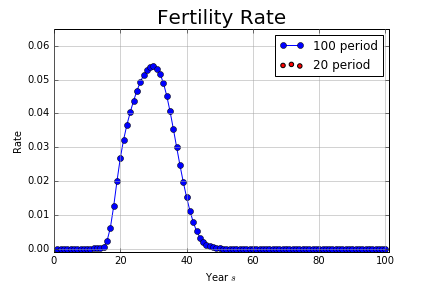
\includegraphics[width=12cm]{fert_rate3}\
    			\textbf{\caption{Fertility Rate for Period 100 and 20}}
		\end{figure}
		
		The above graph is the fertility rate plot for period 100 and 20.\\
	\quad \\
	\end{enumerate}\par
	
\noindent \textbf{\large Problem 2}\par
	\begin{enumerate}[(a)]
		\item \quad \\
		The plot is shown as following:\\
		\begin{figure}[h]
    			\centering
			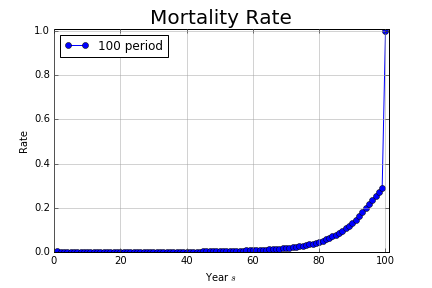
\includegraphics[width=12cm]{mort_rate1}\
    			\textbf{\caption{Mortality Rate for 100 Periods}}
		\end{figure}\par
	
	The above graph is the mortality rate for total period equal to 100 periods.\\
	
		\item \quad \\
		\begin{figure}[H]
    			\centering
			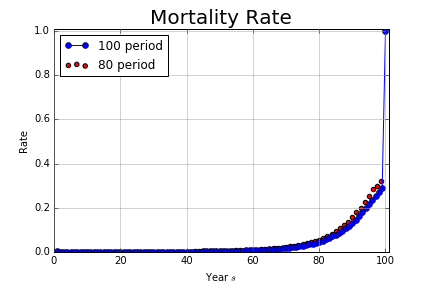
\includegraphics[width=12cm]{mort_rate2}\
    			\textbf{\caption{Mortality Rate for 100 and 80 Periods}}
		\end{figure}
		
		The above graph is the mortality rate plot for period 100 and 80.\\
		
		\item \quad \\
		\begin{figure}[H]
    			\centering
			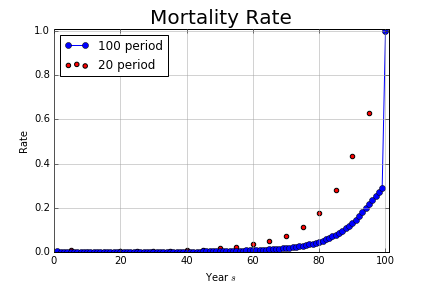
\includegraphics[width=12cm]{mort_rate3}\
    			\textbf{\caption{Mortality Rate for 100 and 20 Periods}}
		\end{figure}
		
		The above graph is the mortality rate plot for period 100 and 20.\\
	\quad \\
	\end{enumerate}\par

\noindent \textbf{\large Problem 3}\par
	\begin{enumerate}[(a)]
		\item \quad \\
		The plot is shown as following:\\
		\begin{figure}[h]
    			\centering
			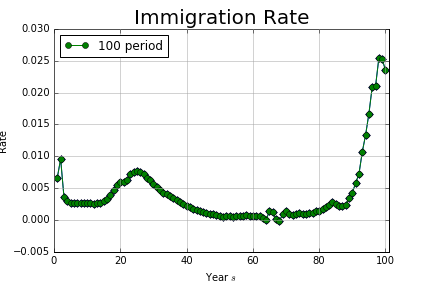
\includegraphics[width=12cm]{immi_rate100}\
    			\textbf{\caption{Immigration Rate for 100 Periods}}
		\end{figure}\par
	
	The above graph is the immigration rate for total period equal to 100 periods.\\
	
		\item \quad \\
		\begin{figure}[H]
    			\centering
			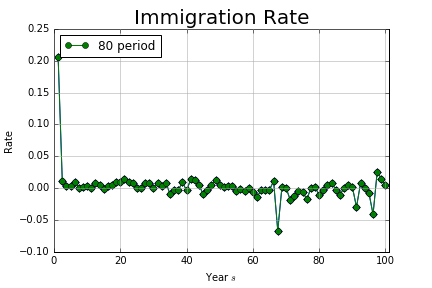
\includegraphics[width=12cm]{immi_rate80}\
    			\textbf{\caption{Fertility Rate for 80 Periods}}
		\end{figure}
		
		The above graph is the immigration rate plot for period 80.\\
		
		\item \quad \\
		\begin{figure}[H]
    			\centering
			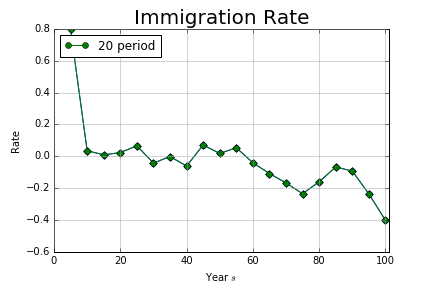
\includegraphics[width=12cm]{immi_rate20}\
    			\textbf{\caption{Fertility Rate for 20 Periods}}
		\end{figure}
		
		The above graph is the immigration rate plot for period 20.\\
	\quad \\
	\end{enumerate}\par
	
\noindent \textbf{\large Problem 4}\par
	\begin{enumerate}[(a)]
		\item \quad \\
		The plot for the stationary population distribution is shown as following:\\
		\begin{figure}[h]
    			\centering
			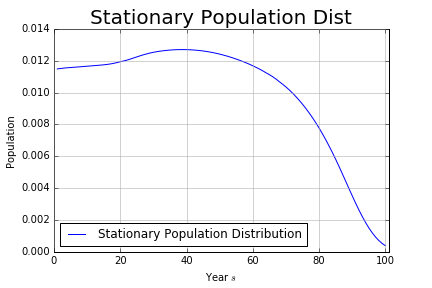
\includegraphics[width=12cm]{pop_ss}\
    			\textbf{\caption{Stationary Population Distribution}}
		\end{figure}\par
	
		\item \quad \\
		\begin{figure}[H]
    			\centering
			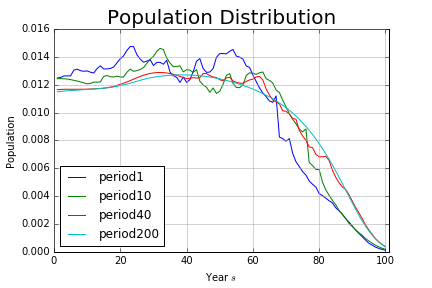
\includegraphics[width=12cm]{pop_dist}\
    			\textbf{\caption{Population Distribution for Multiple Periods}}
		\end{figure}
		
		The above graph is the population distribution  for period 1, 10, 40 and 200.\\
		
		\item \quad \\
		\begin{figure}[H]
    			\centering
			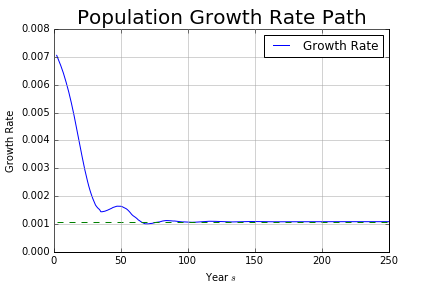
\includegraphics[width=12cm]{pop_growth}\
    			\textbf{\caption{Population Growth Rate Time Path}}
		\end{figure}
		The above plot is the population growth rate time path.
	\quad \\
	\end{enumerate}\par
	

\noindent \textbf{\large Problem 5}\par
	\textbf{Pending}\\

\noindent \textbf{\large Problem 6}\par
	\textbf{Pending}\\




\end{document}







